% % % % % % % % % % % % % % % % % % % % % % % % % % % % % % % % % % % % % % % % % % % %
%                                                                                     %
% Short Sectioned Assignment LaTeX Template Version 1.0 (5/5/12)                      %
% This template has been downloaded from: http://www.LaTeXTemplates.com               %
%                                                                                     %
% Original author:  Frits Wenneker (http://www.howtotex.com)                          %
%                                                                                     %
% Modified by: Fco Javier Sueza Rodríguez (fcosueza@disroot.org)                      %
%                                                                                     %
% Changes:                                                                            %
%	    - Custom Chapters, Sections and Subsections (titlesec package)                %
%           - Document type scrbook (oneside)                                         %
%           - Use babel-lang-spanish package and marvosym                             %
%           - Use hyperref, enumitem, tcolorbox and glossaries packages               %
%           - Use Time New Roman (mathptmx), Helvetic and Courier fonts               %
%                                                                                     %
% License: CC BY-NC-SA 3.0 (http://creativecommons.org/licenses/by-nc-sa/3.0/)        %
%                                                                                     %
% % % % % % % % % % % % % % % % % % % % % % % % % % % % % % % % % % % % % % % % % % % %

%-----------------------------------------------%
%	              Packages                  %
%-----------------------------------------------%

\documentclass[paper=a4, fontsize=11pt, oneside]{scrbook}

% ---- Text Input/Output ----- %

\usepackage[T1]{fontenc}
\usepackage[utf8]{inputenc}
\usepackage{mathptmx}
\usepackage[scaled=.92]{helvet}
\usepackage{courier}
\usepackage[indent=12pt]{parskip}

\usepackage{geometry}
\geometry{verbose,tmargin=3cm,bmargin=3cm,lmargin=2.6cm,rmargin=2.6cm}

% ---- Language ----- %

\usepackage[spanish]{babel}
\usepackage{marvosym}

% ---- Another packages ---- %

\usepackage{amsmath,amsfonts,amsthm}
\usepackage{graphics,graphicx}
\usepackage{titlesec}
\usepackage{fancyhdr}
\usepackage{tcolorbox}
\usepackage{hyperref}
\usepackage{enumitem}
\usepackage[automake]{glossaries}

%--------------------------------------------------------------------%
%                      Customizing Document                          %
%--------------------------------------------------------------------%


% ----------- Custom Chapters, Sections and Subsections -------------- %

\titleformat{\chapter}[display]
			{\bfseries\Huge}
			{Tema \ \thechapter} {0.5ex}
			{\vspace{1ex}\centering}

\titleformat{\section}[hang]
			{\bfseries\Large}
			{\thesection}{0.5em}{}

\titleformat{\subsection}[hang]
			{\bfseries\large}
			{\thesubsection}{0.5em}{}

\titleformat{\subsubsection}[hang]
			{\bfseries\large}
			{\thesubsubsection}{0.5em}{}

\hypersetup{
    colorlinks=true,
    linkcolor=black,
    urlcolor=magenta
}

% ------------------- Custom heaaders and footers ------------------- %

\pagestyle{fancyplain}

\fancyhead[]{}
\fancyfoot[L]{}
\fancyfoot[C]{}
\fancyfoot[R]{\thepage}

\renewcommand{\headrulewidth}{0pt} % Remove header underlines
\renewcommand{\footrulewidth}{0pt} % Remove footer underlines

\setlength{\headheight}{13.6pt} % Customize the height of the header

% --------- Numbering equations, figures and tables ----------------- %

\numberwithin{equation}{section} % Number equations within sections
\numberwithin{figure}{section} % Number figures within sections
\numberwithin{table}{section} % Number tables within sections

% ------------------------ New Commands ----------------------------- %

\newcommand{\horrule}[1]{\rule{\linewidth}{#1}} % Create horizontal rule command


%----------------------------------------------------------------------------------------
%	TÍTULO Y DATOS DEL ALUMNO
%----------------------------------------------------------------------------------------

\title{
\vspace{10ex}
\normalfont \normalsize
\Huge \textbf{Tarea 5: Conversión y Adaptación de Documentos XML}
}
\author{Francisco Javier Sueza Rodríguez}
\date{\normalsize\today}

%----------------------------------------------------------------------------------------
%                                     DOCUMENTO
%----------------------------------------------------------------------------------------
\begin{document}

\maketitle

\thispagestyle{empty}

\vspace{62ex}

\begin{center}
    \begin{tabular}{l l}
        \textbf{Centro}: & IES Aguadulce \\
        \textbf{Ciclo Formativo}: & Desarrollo Aplicaciones Web (Distancia)\\
        \textbf{Asignatura}: & Lenguajes de Marcas y Sistemas de Gestión de la Información\\
        \textbf{Tema}: & Tema 5 - Conversión y Adaptación de Documentos XML\\
    \end{tabular}
\end{center}

\newpage

%\tableofcontents

%\newpage

%\listoffigures

%\newpage

\section{Caso Práctico}
La empresa de reparto LlegaYA, S.L. sigue avanzando. Es momento de utilizar toda nuestra información recogida en formato XML. Realizaremos la conversión y adaptación de documentos XML a otros formatos.

Todo esto nos facilitará exportar nuestra información a la web. Además podremos realizar búsquedas y filtrar la información con los criterios que necesitemos.

\section{Actividades}

\subsection{Enunciado}
En la empresa LlegaYA, S.L. queremos automatizar unos informes mensuales. Nuestro sistema informático registra mensualmente las entregas realizadas que recogemos en el archivo: envio.xml.

Partiendo de la plantilla: envio.xsl, queremos que elabores las siguientes consultas en el formato establecido en cada una.

\begin{enumerate}[label=\Alph*.]
    \item Lista ordenada por precio y apellido de los envíos a Sevilla. Indicar el número de orden (con número), el precio, la moneda, el apellido y el nombre. El orden será de mayor a menor precio y si tienen el mismo precio por orden alfabético de apellido.

    \textbf{Formato:}

    \textbf{1) 33 euros - Sánchez, Carlos.}

    \item Número de envíos urgentes a Cádiz y su porcentaje respecto al total de envíos a Cádiz

    \textbf{Formato}:

    \textbf{Hay 4 envíos urgentes a Cádiz, que suponen el 28.57\% de los 14 envíos totales registrados a Cádiz.}

    \item Lista ordenada (por código de envío) con el tipo de prioridad, la provincia, el nombre y el apellido de todos los envío cuyo nombre comience por 'A' y tengan una prioridad 'Normal', o su apellido contenga una 'a' y la provincia sea 'Almería' o 'Granada'.

    \textbf{Formato}:

    \textbf{1.- (DBD72R - 24\_horas - Granada). Carlos Cano.}

    \item Lista de todas las provincias (ordenadas alfabeticamente) con su número de envíos, ingresos totales (suma de todos sus precios) e ingreso medio.

    \textbf{Formato}:

    \textbf{Almería: 11 envíos. Ingresos totales: 229 euros. Ingreso medio: 20.82 euros.}

    \item Crear una tabla, ordenada por fecha de entrega, de los envíos a Almería. La tabla incluirá las columnas: fecha de entrega, provincia, código de envío y prioridad.

    \textbf{Estilos}:

    La tabla deberá usar los estilos definidos en la plantilla que se proporciona en el ejercicio. Los elementos tabla y las celdas usarán los estilos del descriptores 'table', 'th' y 'td'. La cabecera usará el estilo del descriptor 'th'. Si la prioridad de un envío es 'Urgente' esa celda usará el estilo del descriptor '.urgente'. Si la prioridad de un envío es 'Nocturno' esa celda usará el estilo del descriptor '.nocturno'.

    \textbf{Formato}:

    \begin{figure}[H]
        \centering
        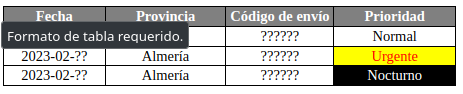
\includegraphics[scale=0.80]{tabla-envios.png}
        \caption{Tabla de Envíos}
    \end{figure}
\end{enumerate}

\subsection{Solución}
En este ejercicios vamos a realizar diversas transformaciones al documento XML de ejemplo para que se nos muestre la información que se nos pide en cada punto. Se incluirá solo el código agregado en cada punto, no la salida.

\begin{enumerate}[label=\Alph*.]
    \item Para resolver este punto, se ha creado un bucle, con \textbf{\textit{<xsl:for-each>}}, donde se han incluido, en primer lugar, dos instrucciones \textbf{\textit{<xsl:sort>}}, una para ordenar por el precio de forma descendente, y otro para ordenar por el apellido, de forma ascendente, por defecto.

    A continuación se ha creado un elemento \textbf{\textit{xs:element}} de tipo \textbf{\textit{<p>}} por cada nodo en el que se ha incluido la información pedida, la cual se ha obtenido con la instrucción \textbf{\textit{xsl:value-of}}, realizando el \textbf{\textit{select}} según la información que se nos pedía, es decir \textbf{\textit{postition()}}, \textbf{\textit{precio}} , \textbf{\textit{apellidos}} y \textbf{\textit{nombre}}.

    \begin{figure}[H]
        \begin{tcolorbox}[sharp corners, colback=yellow!30, colframe=white!20]
            \scriptsize
\begin{verbatim}
<xsl:for-each select="//envio[provincia='Sevilla']">
  <xsl:sort select="precio" data-type="number" order="descending" />
  <xsl:sort select="apellido" />
  <p>
    <xsl:value-of select="position()" />)
    <xsl:value-of select="precio" /> euros -
    <xsl:value-of select="apellido"/>,
    <xsl:value-of select="nombre" />
  </p>
</xsl:for-each>
\end{verbatim}
        \end{tcolorbox}
    \end{figure}

    \item Para resolver este ejercicios se han usado, en primer lugar, \textbf{3 variables}. Una para almacenar
    el \textbf{nombre de la provincia}, otra para el número de \textbf{envios totales} y otra para los \textbf{envíos urgentes}. La variable \textbf{\textit{\$prov}}, que almacena el nombre de la provincia, se han empleado en la
    selección de nodos tanto de \textbf{\textit{\$env\_totales}} como de \textbf{\textit{\$env\_urg}}, de esta forma,
    si quisiéramos mostrar la información de alguna otra provincia, por ejemplo Sevilla, solo habría que cambiar el valor de la variable \textbf{\textit{\$prov}} y se mostrarían los datos correctamente. Además, se ha empleado la función \textbf{\textit{count()}} para el cálculo de la cantidad de envíos en las respectivas variables.

    A continuación se ha creado un elemento de tipo \textbf{\textit{<p>}} mediante \textbf{\textit{xsl:element}} y dentro se han usado diferentes instrucciones de tipo \textbf{\textit{xsl:value-of}} para mostrar la información requerida. Cabe mencionar el caso del \textbf{cálculo del porcentaje}, donde se ha usado en el \textbf{\textit{select}} la función \textbf{\textit{format-number}} para dar un formato adecuado a la salida del cálculo del porcentaje, ya que por defecto muestra demasiados decimales.

    \begin{figure}[H]
        \begin{tcolorbox}[sharp corners, colback=yellow!30, colframe=white!20]
            \tiny
\begin{verbatim}
<xsl:variable name="prov" data-type="text" select="'Cádiz'" />
<xsl:variable name="env_urg" select="count(//envio[provincia=$prov and prioridad='Urgente'])" />
<xsl:variable name="env_total" select="count(//envio[provincia=$prov])" />

<xsl:element name="p">
  Hay <xsl:value-of select="$env_urg" /> envíos urgentes a <xsl:value-of select="$prov" />,
  que supone el  <xsl:value-of select="format-number(($env_urg div $env_total) * 100, '#.##')" />%
  del los <xsl:value-of select="$env_total" /> envíos totales registrados a
  <xsl:value-of select="$prov" />.
</xsl:element>
\end{verbatim}
        \end{tcolorbox}
    \end{figure}

    \item
\end{enumerate}




% Bibliography

%\newpage

%\bibliography{citas}
%\bibliographystyle{unsrt}

\end{document}